\section{Methodology} \locallabel{sec:methodology}

In this section we describe the classes in our study, explain the concept of a
feedback delay, and briefly provide an overview of our system architecture.

\subsection{Classes}

\begin{figure}[!t]
\centering 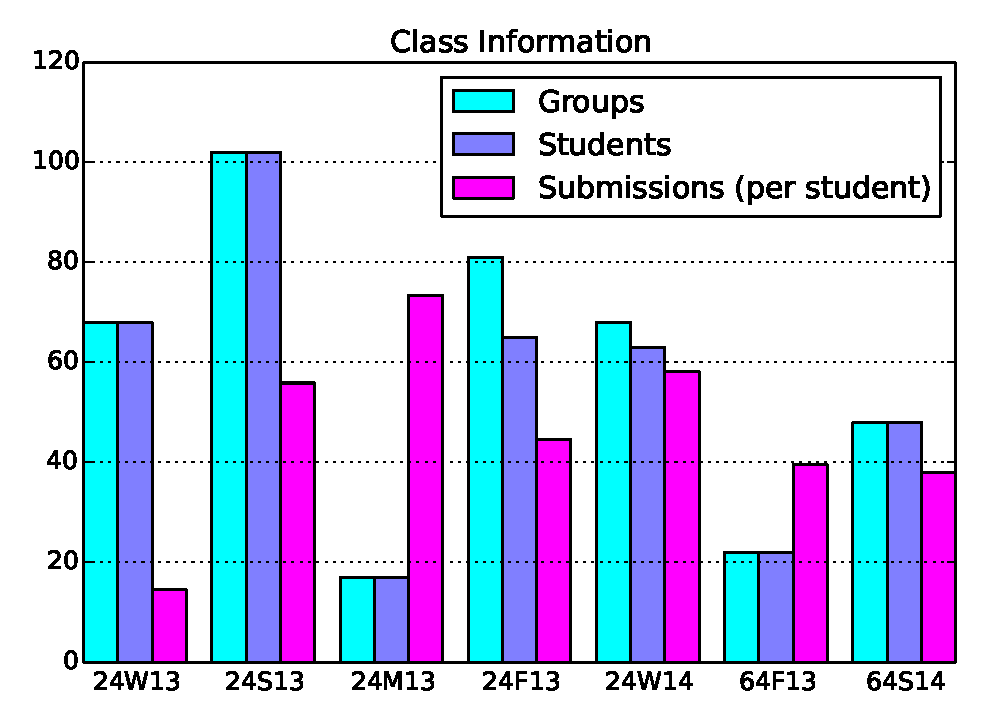
\includegraphics[width=3.3in]{graphs/Class_Information.eps}
\caption{Visualizes the number of groups, students, and average number of
  submissions by student for each of the seven classes in the study.}
\locallabel{fig:class_info}
\end{figure}

Our study involves seven instances of two UCSB computer science courses from
Winter Quarter 2013 through Spring Quarter 2014. The first course, \emph{CS24},
is the second required course in UCSB's lower division computer science
curriculum and builds upon students' prior knowledge of \emph{C} in order to
introduce them to data structures, and object oriented programming in
\emph{C++}. The second course, \emph{CS64}, is a lower division computer
architecture course that educates students on assembly programming and the
basics of computer architecture, including digital design. In total, there are
five instances of \emph{CS24}, and two instances of \emph{CS64} represented in
this study. A single instructor taught \cm[24]{13} and \cf[24]{13}, and all
others were taught by another individual instructor. All classes were taught
during a ten-week quarter including \cm[24]{13}, the only summer instance in
the study.

While our feedback and assessment system supports both programming assignments
and \emph{fill in the blank}-type assignments, we only consider programming
assignments in this study. Figure~\localref{fig:class_info} provides useful
information for each class in this study. The purple bars indicate the number
of consent giving students that made at least one submission, and the pink bars
indicate the average number of submissions made by each student. Finally, the
cyan bars indicate the number of unique groups that made at least one
submission to any of a class's assignments. Most students formed the same group
across assignments, however, that was not a requirement.

We distinguish between students and groups because our feedback and assessment
system enforces an instructor defined maximum group size per assignment. When
the maximum group size is more than one, students are able to join into groups
with other students up to the maximum group size. With regard to consent giving
students, we only include submissions in this study if we have consent from all
group members. This grouping functionality was only introduced in September
2013, therefore it was only utilized by classes \cf[24]{13} and \cw[24]{14}. In
addition to a few students changing groups between assignments, a few worked
independently on assignments and thus are counted as a single-student group.

Two classes have an average number of submissions which stand out. First, the
average number of submissions is low for \cw[24]{13} due to only using the
feedback and assessment system for half of the quarter. In the first half of
the quarter, the students made submissions using an archaic submission system
that provides no feedback. Second, the average number of submissions per
student for \cm[24]{13} is relatively high due to students making post-deadline
submissions as discussed in Section~\localref{sec:deadline}.


\subsection{Feedback Delay} \locallabel{sec:delay}
The primary educational purpose of a real-time feedback and assessment system
is to provide feedback to students so that they may iteratively achieve mastery
on their assignments. The use of these systems has positive side effects
including reducing assessment time while increasing assessment equitability. As
many instructors have previously observed, however, student usage of real-time
feedback and assessment systems may result in dependency upon the system. This
dependency could inhibit students from expanding their knowledge of
compilation, execution, testing, and debugging processes.

Researchers have made various attempts to solve this dependency
problem. Web-CAT ensures students develop testing skills by requiring students
to submit test cases along with their assignment
code~\cite{Edwards:2003:RCS:949344.949390}. While this approach appears
successful to help students develop testing skills, it is not suitable for our
purposes because it would require a change to our lower-division curriculum in
order to emphasize testing. In another attempt, Marmoset restricts the
frequency of running a subset of assignment test cases, called \emph{release
  tests}, through a limited number of \emph{release tokens}. While this notion
of feedback reduction was also meant to encourage students to start assignments
earlier, \spacco{} indicated that the release tokens were seldom
used~\cite{Spacco:2013:TIP:2462476.2465594}. This result suggests that the
standard assignment test cases, which students could always get feedback from,
provided sufficient coverage for students to complete their
assignments. Furthermore, this observation may be indicative of a problem with
requiring instructors to properly partition their test cases.

We built our system in order to take an alternative approach that can be
transparently utilized by UCSB's existing computer science curriculum, and
requires minimal assignment configuration by instructors. Our approach is to
introduce a configurable per-assignment feedback delay for submissions that
occur within a short period of time to each other. For example, if the feedback
delay is configured as five minutes, then students will receive immediate
feedback from only one new submission in any five-minute window. Alternatively,
if students make submissions exactly five minutes or more apart, they will
never experience any delay in receiving feedback. Our hypothesis was, that as
the feedback delay increased, students would spend more time testing their
assignments prior to submission, with the result of both lengthening the time
between submissions, and inflating the improvement in score between
submissions.

In attempt to measure the effects of the feedback delay on student submission
behavior, we increased the feedback delay in five-minute increments for each
subsequent assignment in three of our classes: \cs[24]{13}, \cm[24]{13}, and
\cf[24]{13}. In all other classes, the feedback delay was not intentionally
altered between assignments. The impact of the feedback delay is detailed in
Section~\localref{sec:sub_impact} and Section~\localref{sec:session_impact}.


\subsection{The Feedback and Assessment System}

\begin{figure}[!t]
\centering 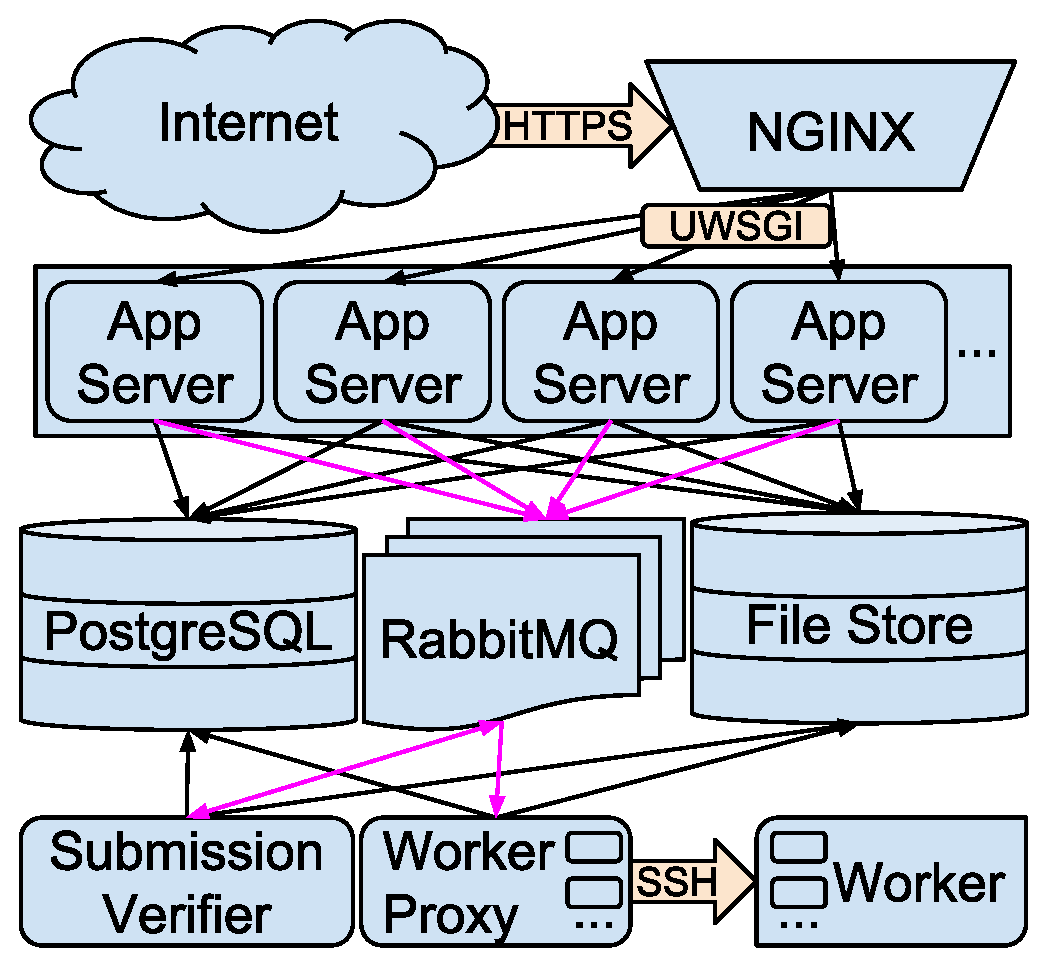
\includegraphics[width=3.3in]{graphs/architecture.eps}
\caption{Provides an overview of the system architecture and how components
  interact. Pink lines indicate messages being passed to and from the RabbitMQ
  service. Note that each \emph{worker} runs in a separate isolated
  environment.}
\locallabel{fig:architecture}
\end{figure}

In this section we describe our rationale for creating a new real-time feedback
and assessment system, as well as provide a high-level overview of the system's
architecture.

\subsubsection{Rationale}
We chose to design and build our own system for a number of reasons. First, and
foremost, we wanted to have a system that was easy to adopt into existing
curriculum in order to encourage more instructors to use the system in their
classes. We specifically designed our system to match existing department
submission and assessment work flows.

In a similar vein, we designed the \emph{workers}, processes that execute
student code as described in detail in Section~\textbf{Architecture Overview},
such that they would run on existing lab machines in order to provide a
consistent test and development environment without requiring additional
resources from the technical support department. Having a consistent
environment also contributes to instructor adoption of the
system. Additionally, by utilizing existing machines we are able to provide
significant \emph{worker} redundancy making it possible to have zero issues
with the most volatile part of the system at no additional cost to our
department.\footnote{A redesign and implementation of this component was
  required in order to achieve this result. The system has since run with a
  peak activity for three months without a single issue.}

Finally, by building our own system we could ensure that we had total knowledge
of all components of the feedback and assessment system. This knowledge allows
us to easily adjust and control the various aspects of the submission,
feedback, and assessment processes as necessary for both current research and
future research efforts.

In designing the feedback and assessment system we had two primary goals:

\begin{itemize}
\item Students should be able to make assignment submissions from either the
  web interface or lab machine terminals with little or no instruction.
\item To reduce the overall assessment time for instructors and teaching
  assistants, including the time to prepare assignment test cases.
\end{itemize}

We believe the first goal was met due to the absence of complaints regarding
usability of the system by the more than 300 students who used the system. We
confirmed we met the second goal when, on more than one occasion, an instructor
had to find additional work for their teaching assistants due to a significant
reduction in assessment time.


\subsubsection{Architecture Overview}
Figure~\localref{fig:architecture} provides a diagram of the system
architecture. In a nutshell, the primary interface to the system for
instructors, teaching assistants, and students is their web browser. An
\emph{NGINX} web server distributes Internet HTTPS requests across a number of
\emph{app servers} that run the actual web service code. The system data is
stored either in a \emph{PostgresSQL} database, or deduplicated via an on-disk
\emph{file store}. A \emph{submission verifier} process exists that checks new
submissions for proper files prior to triggering one or more relatively
resource expensive build and test jobs. A one-to-one mapping exists between a
\emph{worker proxy} and a \emph{worker} where the \emph{worker proxy} is
responsible for selecting a machine for the \emph{worker} to run on, initiating
the build and test processes via the \emph{worker}, and comparing the results
generated by the \emph{worker} to the assignment's expected
results. \emph{RabbitMQ} is used to pass messages that trigger the jobs run by
the \emph{submission verifier} and the \emph{worker proxies}.

All of the components, save for the \emph{workers}, run on a single machine as
we have yet to experience any web service related performance issues. While
there is a single point of failure at that machine, a manual failover to the
development machine requires only minutes, with at worst an hour of data
loss. Moreover, providing redundancy on these components is trivial because the
system was designed to support this expansion pending available hardware.

In addition to the primary web interface, any number of additional interfaces
can be created that communicate through the system's REST API. For instance,
two such interfaces exist which both simplify a distinct task for command-line
savvy users of the system:

\begin{itemize}
\item A submission creation program was written that creates a submission for a
  student by uploading the specified submission files. This program was written
  to provide transparency with the archaic non-feedback submission process.
\item An assignment test case synchronization program was written that allows
  an instructor or teaching assistant to quickly synchronize an assignment on
  the system with the contents of a directory on their local machine. This
  program dramatically decreases the time to configure an assignment because,
  while it is easy to add test cases through the web interface, it can be
  tedious if there are more than a handful of them.
\end{itemize}
